% ****** Start of file aipsamp.tex ******
%
%   This file is part of the AIP files in the AIP distribution for REVTeX 4.
%   Version 4.1 of REVTeX, October 2009
%
%   Copyright (c) 2009 American Institute of Physics.
%
%   See the AIP README file for restrictions and more information.
%
% TeX'ing this file requires that you have AMS-LaTeX 2.0 installed
% as well as the rest of the prerequisites for REVTeX 4.1
%
% It also requires running BibTeX. The commands are as follows:
%
%  1)  latex  aipsamp
%  2)  bibtex aipsamp
%  3)  latex  aipsamp
%  4)  latex  aipsamp
%
% Use this file as a source of example code for your aip document.
% Use the file aiptemplate.tex as a template for your document.
\documentclass[%
 aip,
 % apl,
% jmp,%
% bmf,%
% sd,%
% rsi,%
 amsmath,amssymb,
% preprint,%
 reprint,%
% author-year,%
% author-numerical,%
 floatfix,%
]{revtex4-1}

\usepackage[utf8]{inputenc}
\usepackage{tikz}
\usepackage{graphicx}% Include figure files
\usepackage{dcolumn}% Align table columns on decimal point
\usepackage[T1]{fontenc}
\usepackage{bm}% bold math
\usepackage{mathptmx}
\usepackage{siunitx}
\usepackage{textcomp}
\usepackage{gensymb}
\usepackage{float}
%\usepackage[mathlines]{lineno}% Enable numbering of text and display math
%\linenumbers\relax % Commence numbering lines
\usetikzlibrary{arrows,decorations.markings,decorations.pathmorphing, patterns,shapes}

\begin{document}

\preprint{AIP/123-QED}

\title[]{The Double Pendulum:\\Creating a Better Baseball Bat}
%\thanks{Footnote to title of article.}

\author{Jared Baur}
%\altaffiliation[Also at ]{Physics Department, Occidental College.}%Lines break automatically or can be forced with \\

\date{\today}% It is always \today, today,
             %  but any date may be explicitly specified

\begin{abstract}
	To be written later.
\end{abstract}

\maketitle

% \onecolumngrid

\section{\label{sec:level1}Introduction}

The double pendulum is a classic example of chaotic motion\cite{Shinbrot1992}. The trajectories of various trials will show that the motion of a double pendulum is highly unpredictable. The chaos in a classic double pendulum is described by Equation 1. The exponent $\lambda$ is a positive constant, $\Delta x$ is the trajectory of the bottom arm of the pendulum, and $t$ is time. For small times $t$, the trajectories are relatively the same, however for increasing times, the trajectories exponentially increase in distance from trial to trial.
\begin{equation}
	\Delta x(t) \sim \Delta x(t_0) e^{\lambda t}
\end{equation}

\begin{figure}
	\centering
	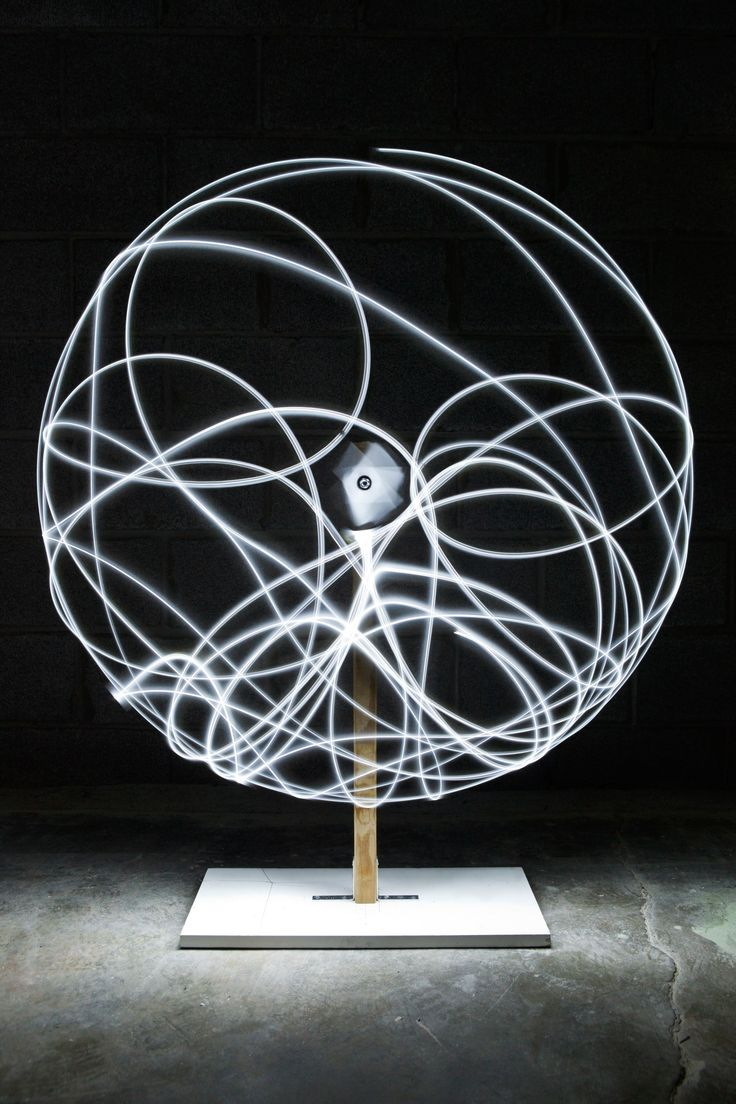
\includegraphics[scale=0.25]{lights.jpg}
	\caption{Chaos in a double pendulum. This figure depicts the trajectory of the end of the bottom arm in the double pendulum. The light is traced along the route of the bottom arm. As seen, there is no evident pattern in the bottom arm's trajectory.}
\end{figure}

The double pendulum is used in real life situations such as in double-trailer trucks (officially known as “long combination vehicles”) where two large-wheeled vehicles are combined at a hinge point. These vehicles are essentially semi-trucks with two trailers attached instead of one. The swinging motion in sports is also a common instance of a double pendulum. For this paper, the double pendulum will be compared to a baseball swing. In a baseball swing, a bat (striking implement) is used in conjunction with the arms to strike a baseball. In general, the arms are held up and back from the player's head, with the bat pointed upwards. The arms initiate the swing, moving towards the center of the player's body; the bat follows the arms, and then swings through as the transfer of energy from the arms to the bat occurs. This motion occurs mostly in the horizontal plane, but nonetheless acts as a double pendulum with the player's arms and the bat as the upper and lower “arms” of the pendulum, respectively.

Since the swing of a baseball bat only occurs once per trial (does not swing back and forth and time $t$ is relatively low), this motion is equivalent to the first half cycle of a double pendulum swing. Thus, the chaotic motion prevalent in classic double pendulums will not be applicable for the purpose of the baseball swing.

Although the focus of this paper will be on the baseball swing, the double pendulum motion can be applied to the motion of a swing of a baseball bat, golf club, tennis racquet, or any other “swinging” motion that occurs with a striking implement. The goal of this paper will be to quantitatively describe the double pendulum in the context of a baseball swing and determine whether all of the energy in the striking implement can be transferred to the ball on impact. From this, we will decide whether we can design a baseball bat or ball that would allow for this perfect transfer of energy to occur.

\section{\label{sec:level2}Equations of Motion}

Describing the motion of a double pendulum has been argued as highly complicated\cite{Jorgensen1970}. For this reason, Lagrangians have been used in past studies to represent this motion. However, when we look at the forces on each arm of the pendulum with respect to each arm's center of mass, Newtonian equations of motion can be used to describe the motion.

Figure 2 depicts the components in a simple double pendulum. The $x,y$ axes for position and forces are shown in the figure. The upper arm of the pendulum is the first arm attached to a fixed axis $A$. This arm has length $L_1$, center of mass at point $G_1$, and distance to its center of mass $h_1$ (measured from point $A$). This arm makes an angle $\theta$ with the vertical axis and has a gravitational force acting on its center of mass equal to $M_1 g$, where $M_1$ is the mass of the arm and $g$ is the acceleration due to gravity.

The second arm (lower arm) rotates on a “fixed” axis at point $B$. If we isolate the second arm from the system, it would rotate about point $B$ as if it were fixed, however point $B$ is rotating around point $A$ since it is at the end of the first arm. The second arm has a length $L_2$ and its center of mass at point $G_2$, a distance of $h_2$ away from point $B$. The arm makes an angle of $\phi$ with the vertical axis and has a gravitational force of $M_2 g$ acting on its mass $M_2$. Point C is the end of the second arm, and will act as a point of interest for our paper as we track the trajectory of this point. The velocity vector $V$ is the direction of motion for the second arm's center of mass through the swinging of a double pendulum. 
\begin{figure}
	\centering
	\begin{tikzpicture}
		\node [inner sep=0pt,above right]
		{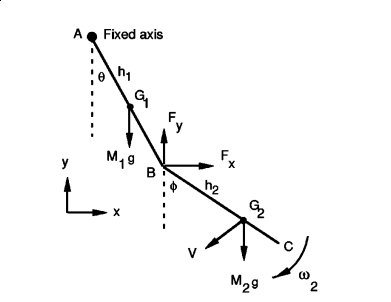
\includegraphics[scale=0.6]{equationsofmotion.png}};

		\draw[<->] (2,2.85) -- (0.5,5.5);
		\node (none) at (1,3.8) {$L_1$};

		\draw[<->] (5.5,2.85) -- (7.9,1.3);
		\node (none) at (6.9,2.4) {$L_2$};

	\end{tikzpicture}
	\caption{The components in a double pendulum. Since the equations that describe a double pendulum can be rather confusing, we use the center of mass $G_1$ and $G_2$ to describe the forces acting on the pendula arms.}
\end{figure}

We start writing our equations of motion by describing the coordinates of our center of mass on the second arm. We want the coordinates of the center of mass since we will write our forces with respect to that (as opposed to point C). Point $G_2$ is described in Equation 2, where the first half of the equation is the $x$ component and the second half is the $y$ component. The $y$ component is negative since the double pendulum's origin at $(x,y)=(0,0)$ is assumed at point $A$.

\begin{equation}
	G_2(x,y) = \Big([L_1 \sin{\theta} + h_2 \sin{\phi}],  [- L_1 \cos{\theta} - h_2 \cos{\phi}]\Big)
\end{equation}

The velocity of point $G_2$ is found by using the angular velocity of the entire first arm, $\omega_1$, and combining it with the angular velocity of the second arm, $\omega_2$. The components of this velocity are found by multiplying the angular velocities against the distance to point $G_2$. For the $x$-direction, we take $-L_1 \cos{\theta}$ for the first arm and $-h_2 \cos{\phi}$ for the second arm. Likewise for the $y$-direction, we take $-L_1 \sin{\theta}$ and $-h_2 \sin{\phi}$ for the first and second arms, respectively. These components are oriented negatively since the arm is moving in the negative $x$- and $y$-directions. The velocities $V_x$ and $V_y$ for point $G_2$ are described in Equations 3 and 4.

\begin{equation}
	V_x = \frac{dx}{dt} = -L_1 \omega_1 \cos{\theta} - h_2 \omega_2 \cos{\phi}
\end{equation}

\begin{equation}
	V_y = \frac{dy}{dt} = -L_1 \omega_1 \sin{\theta} - h_2 \omega_2 \sin{\phi}
\end{equation}

The forces on center of mass point $G_2$ are found by taking the derivatives of Equations 3 and 4. Newton's second law $\sum \bold{F} = m \bold{a}$ is used to describe the sum of forces acting on the double pendulum. For the force in the $x$-direction, the only force applied to $G_2$ is the force from the upper arm pulling on the lower arm. For the $y$-direction, the upper arm as well as force due to gravity act on the lower arm. The $x$- and $y$-components of force are given by Equations 5 and 6.

\begin{equation}
	\begin{aligned}
		F_x & = M_2 \frac{d V_x}{dt} \\
		    & = -M_2 \bigg [ L_1 \cos{\theta} \frac{d \omega_1}{dt} + L_1 \omega_1^2 \sin{\theta} \\
		    & + h_2 \cos{\phi} \frac{d \omega_2}{dt} + h_2 \omega_2^2 \sin{\phi} \bigg ]
	\end{aligned}
\end{equation}

\begin{equation}
	\begin{aligned}
		F_y - M_2 g & = M_2 \frac{d V_y}{dt}\\
		   & = -M_2 \bigg [ L_1 \sin{\theta} \frac{d \omega_1}{dt} - L_1 \omega_1^2 \cos{\theta} \\
		   & + h_2 \sin{\phi} \frac{d \omega_2}{dt} - h_2 \omega_2^2 \cos{\phi} \bigg ]
	\end{aligned}
\end{equation}

These derived equations are for a generic double pendulum that falls in a vertical fashion. In order to apply this concept to the swing of a baseball bat, we will use the torques on the pendula components. The terminology we will use for the upper and lower components of the pendulum will be the “arm” and “rod”, respectively. In a baseball swing, we assume that the upper body musculature applies a torque $C_1$ to the arm and a torque $C_2$ to the rod of the pendulum. These torques originate from the equal and opposite muscle and joint reaction forces from the shoulder and elbow joints\cite{Cross2005} (points $A$ and $B$, respectively). The net torque acting on the arm is given using the generic equation $\sum \bold{\tau} = \bold{I} \frac{d \bold{\omega}}{dt}$, where $\tau$ is the net torque, $I$ is the moment of inertia, and $\omega$ is the angular velocity. With torques $C_1$ and $C_2$ on the arm and rod, the rod exerts an equal and opposite torque $-C_2$ on the arm. There is also a clockwise torque on the arm about point $A$ in the form of $F_x L_1 \cos{\theta} + F_y L_1 \sin{\theta}$. Thus, the torque acting on the arm is given by Equation 7.

\begin{equation}
	\begin{aligned}
		\sum \tau_{\text{arm}} & = I_1 \frac{d \omega_1}{dt} \\ 
			  & = C_1 - C_2 + M_1 g h_1 \sin{\theta} + F_x L_1 \cos{\theta} + F_y L_1 \sin{\theta}
	\end{aligned}
\end{equation}

The torque acting on the rod's center of mass is given in Equation 8. The arm applies no torque to the rod. We solve for the torque on the center of mass for the rod since we are interested in this point as it pertains to the transfer of energy (described in the coming sections).

\begin{equation}
	\begin{aligned}
		\sum \tau_{\text{rod}} & = I_{c.m.} \frac{d \omega_2}{dt} \\ 
			  & = C_2 + F_x h_2 \cos{\phi} + F_y h_2 \sin{\phi}
	\end{aligned}
\end{equation}

Substituting in Equations 5 and 6, we get a complete description of the torque on the system (Equation 9). The angle $\beta$ is the difference between $\phi$ and $\theta$ ($\beta = \phi - \theta$), $A=I_1+M_2L_1^2$, $B=M_2h_2L_1$, and $I_2=I_{c.m.}+M_2h_2^2$.

\begin{equation}
	\begin{aligned}
		C_1 - C_2 = & A \frac{d \omega_1}{dt} + B \cos{\beta} \frac{d \omega_2}{dt} + B \omega_2^2 \sin{\beta} \\
			    & -(M_1 h_1 + M_2 L_1) g \sin{\theta}\\
		C_2 = & I_2 \frac{d \omega_2}{dt} + B \cos{\beta} \frac{d \omega_1}{dt} \\
		      & -B \omega_1^2 \sin{\beta} -M_2 h_2 g \sin{\phi}
	\end{aligned}
\end{equation}

% *to-do:verify equations*

It is difficult to parse Equation 9 for context of the nature of our system. To simplify the equation, we use initial conditions that are relevant to our baseball swing. Referring to Figure 3, we have the conditions $\theta=90\degree$, $\phi=180\degree$, and $\beta=90\degree$. We also apply the initial condition that $C_1 = C_2 = 0$, since initially, the upper body musculature is not applying a torque to the arm or the rod components of the pendulum. Applying the initial conditions to Equation 9, we get a simplified version that is more applicable to the baseball swing. This simplified version is presented in Equation 10.

\begin{equation}
	\begin{aligned}
		M_1 g h_1 - F_y L_1  & = I_1 \frac{d\omega_1}{dt} \\
		F_x h_2 & = -I_{c.m.} \frac{d\omega_2}{dt}
	\end{aligned}
\end{equation}

\begin{figure}
	\centering
	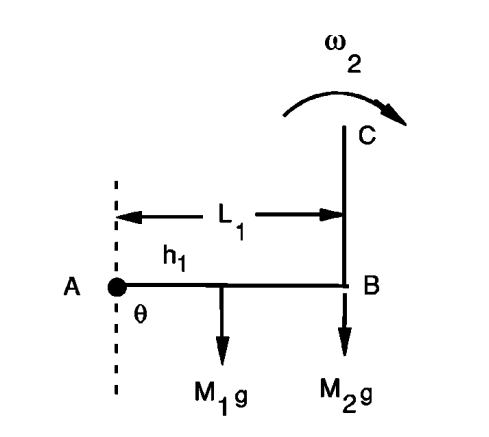
\includegraphics[scale=0.5]{wristcock.png}
	\caption{Initial conditions of the double pendulum with $\theta=90\degree$, $\phi=180\degree$, and $\beta=\phi-\theta=90\degree$. These initial conditions accurately simulate the baseball swing, since the arms are most often at a $90\degree$ angle with the bat right before a swing.}
\end{figure}

In the position depicted in Figure 3, the swing has not yet begun, so we are at time $t=0$. At this time, the angular velocities of the arm and rod are $\omega_1=\omega_2=0$. This means that Equation 10 can be further simplified into the initial angular accelerations of the arm and rod (given in Equation 11).

\begin{equation}
	\begin{aligned}
		\frac{d\omega_1}{dt} & = \frac{g}{A}(M_1 h_1 + M_2 L_1) \\
		\frac{d\omega_2}{dt} & = 0
	\end{aligned}
\end{equation}

\section{\label{sec:level3}Experimental Results}

An experimental double pendulum was constructed in the study by Cross et al.\cite{Cross2005} from two $0.30$ meter length aluminum bars, the upper bar of mass $109.3$ grams and the lower bar of mass $25.0$ grams. A mechanical stop was implemented, which kept the $\beta$ angle between the arm and the rod of the pendulum at $90 \degree$ for the initial stage of the swing. The mechanical stop implemented is a small bolt placed inbetween the arm and the rod that prevents the $\beta$ angle from falling below $90\degree$, shown in Figure 4. Contact between the bolt and the end of the arm applies a force $F$ on the rod. An equal and opposite force is incident on the arm at the “hinge” location. These forces do not significantly contribute to the overall acceleration of the rod through its swinging motion. After the arm swings through to about $\theta = 75\degree$, $15\degree$ less than its initial angle, the $\beta$ angle increases past $90\degree$, thus the bolt loses contact with the rod and this contact force is nonexistent.

\begin{figure}[H]
	\centering
	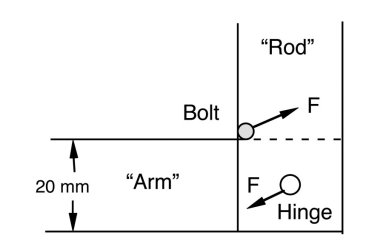
\includegraphics[scale=0.4]{stopmechanism.png}
	\caption{The stop mechanism that enables an initial $\beta$ angle of $90\degree$ at the initial swing position. The stop mechanism is a rod placed at the hinge of the arm and the rod that applies a force to the rod. An equal and opposite force is applied to the arm.}
\end{figure}

The stop mechanism is a simulation of actual tendons in the human body that pull on the bone to place joints and limbs in specific positions. In the case of the baseball swing pendulum, the stop mechanism simulates tendons in the forearm and wrist that pull the wrist into a cocked position, holding the bat at a $90\degree$ angle to the arms. A visual representation of this is given in Figure 5.

\begin{figure}[H]
	\centering
	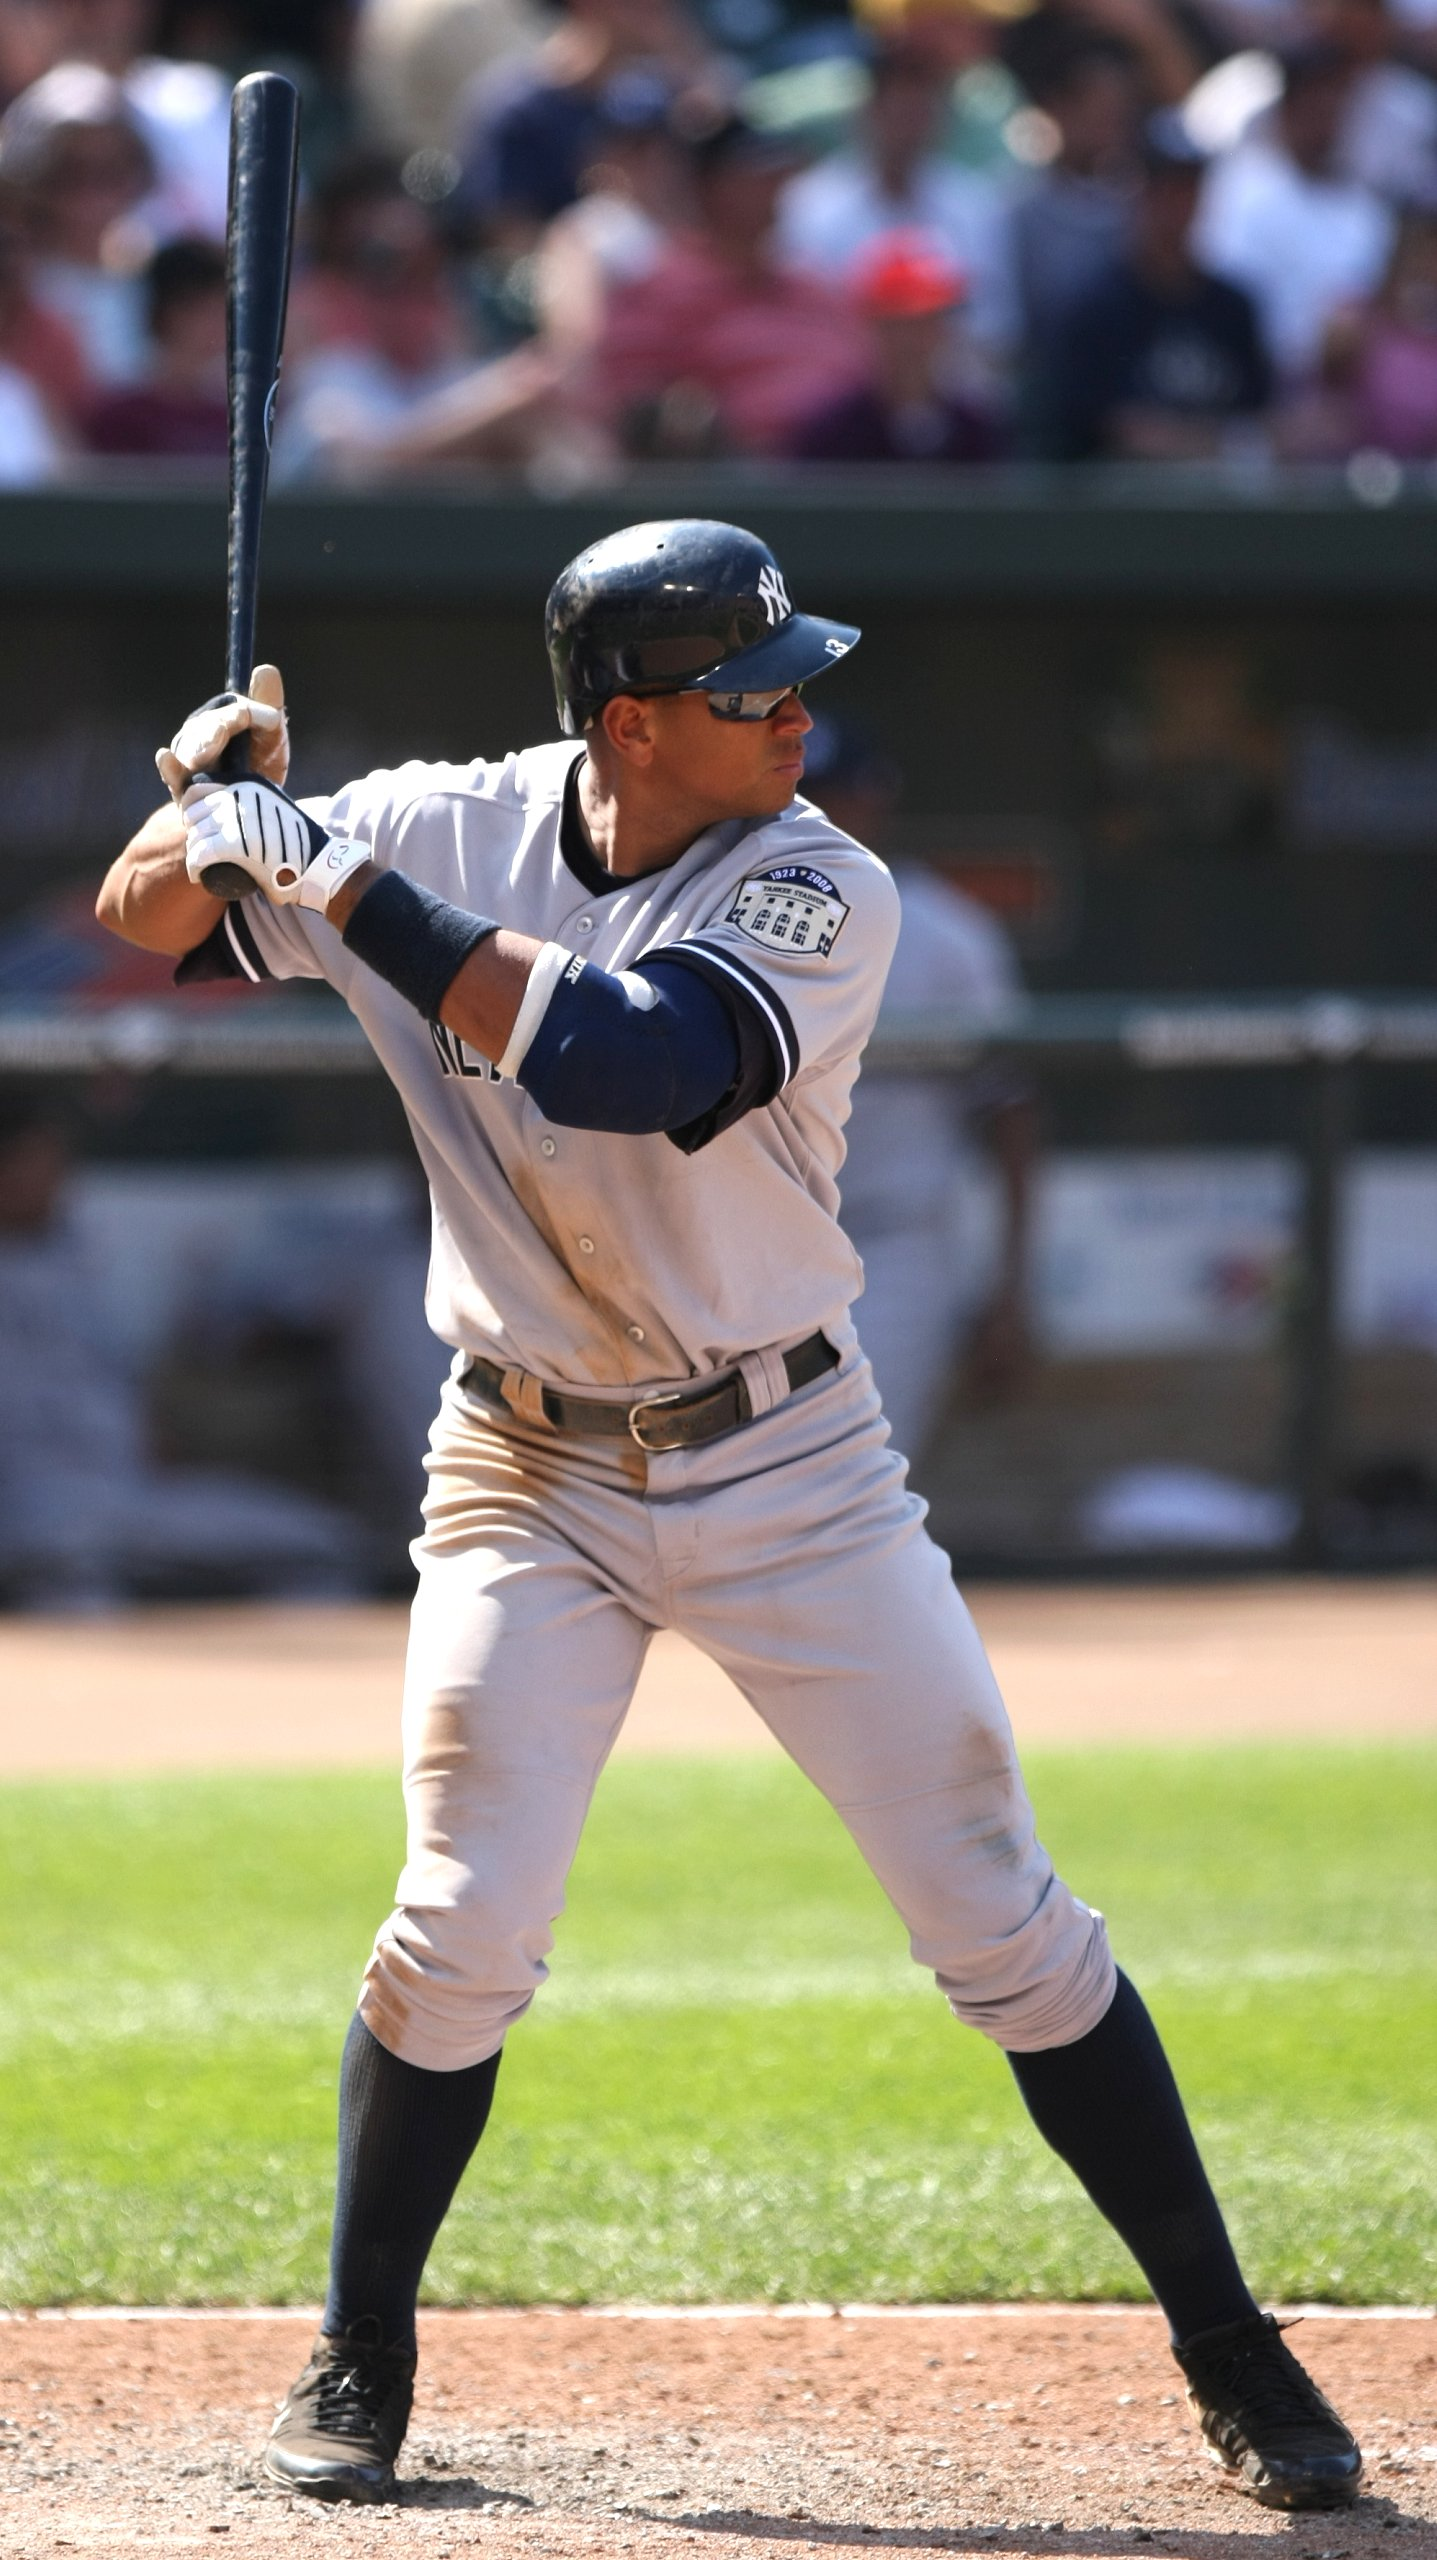
\includegraphics[scale=0.1]{arod.jpg}
	\caption{A visual of the real life $\beta=90\degree$ angle between the “arm” and “rod” (for the double pendulum) or arms and bat (for the baseball player).}
\end{figure}

An extra 51.3 g mass was attached to near the end of the rod to increase the moment of inertia of the rod. This added mass, however, creates an unrealistic scenario in which the arm mass to rod mass ratio is too small. In baseball, a realistic arm to rod mass ratio is around 6:1. This added mass lowers the ratio. The increased moment of inertia was simply desired for experimental variability. Trials of the double pendulum swing were ran under the four following conditions:

\begin{itemize}
	\item Without the stop mechanism and without the added 51.3 g mass,
	\item Without the stop and with the added mass,
	\item With the stop and without the added mass,
	\item With the stop and with the added mass.
\end{itemize}



These trials were ran with the afformentioned initial conditions (Figure 3); video software was used to track the $(x,y)$ positions of points of interest for our double pendulum through its swing. The trajectory of point $C$ (the end of the rod) is shown in Figure 6. The chaos that was mentioned earlier in this paper can be seen in Figure 6 to be irrelevant. Since only the first half-cycle of the pendulum swing is representative of the baseball swing, the time $t$ (Equation 1) needed for chaos to become significant is too small. Figure 6 proves that the double pendulum swing is reproducable for this experiment. The graph on the right in Figure 6 is the angular velocity of the arm ($\omega_1$) and the angular velocity of the rod ($\omega_2$) for the same swings used to produce the graph of the trajectories of point $C$. The velocities can be viewed as “coupled”, that is, they react to each other strongly. When the angular velocity of the arm is at a minimum, the angular velocity of the rod is at a maximum. This means that momentum is being transferred efficiently into the rod. 

\begin{figure}[H]
	\centering
	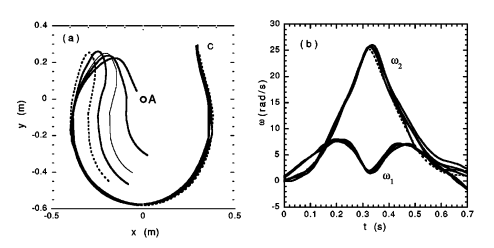
\includegraphics[scale=0.4]{trajectory.png}
	\caption{The trajectory of point $C$ through the full half-cycle swing of the experimental double pentulum. As seen, the trajectories are the same through the greater majority of this motion. The angular velocities of the arm and rod are coupled; the rod is at a peak angular velocity when the arm is at its minimum.}
\end{figure}

The same trials were ran for the four conditions previously mentioned. These results are shown in Figure 7. *to-do: talk about differences between trials*

For all trial conditions, the maximum rod angular velocity occurs during the point of the minimum arm angular velocity. In the case with no stop mechanism and no extra 51.3 g mass, the minimum arm angular velocity goes to zero and the maximum rod angular velocity is the highest out of all trial conditions. For the trial with no stop mechanism and the extra mass, the minimum angular velocity for the arm dips below zero, which means that the arm travels backwards in its motion as the energy is transferred from arm to rod. This is unrealistic as it relates to the baseball swing since the arms in the baseball swing do not travel backwards; they actually continue moving forward at a decreased velocity (nonzero velocity). In the trial with the stop mechanism and no added mass (the most realistic case due to the accurate arm to rod ratio and stop mechanism), the minimum arm angular velocity does not go to zero. For the trial with the stop mechanism and the added mass, the minimum arm angular velocity dips below zero. There is another moment in this swing where the arm and rod share their minimum and maximum angular velocity, however the arm is now at the maximum and the rod is at the minimum. For both trials with the stop mechanism, the arm and rod have the same angular velocity for about the first 0.2 seconds. This is due to the stop mechanism holding the arm and the rod in the same position relative to one another as they swing through their first cycle. The added mass to the rod increases the coupling between the arm and the rod since the arm and rod swap velocity and direction with one another. If the mass of the rod $M_2$ were to go to zero, the coupling would also go to zero. If the mass of the arm $M_1$ were to go to zero, the coupling would increase. This situation is similar to a double pendulum in which the upper arm of the pendulum is a string ($M_1 \approx 0$), which has been proven to have high coupling. Increased coupling between the arm and the rod produces increased angular velocity of the rod, which improves the performance of the rod's ability to hit a ball further. An increased velocity improves the ability for the rod to transfer the maximum amount of momentum into the ball. Unfortunately, the stop mechanism does decrease this coupling, however this limitation provides the most realistic swing in context with the baseball swing. The highest angular velocity of the rod also occurs when the angular velocity of the arm goes to zero ($\omega_1 \rightarrow 0$). In the case where $\omega_1 = 0$ at the arm's minimum, none of the kinetic energy is retained in the arm and all of it is transferred to the rod.

\begin{figure}[H]
	\centering
	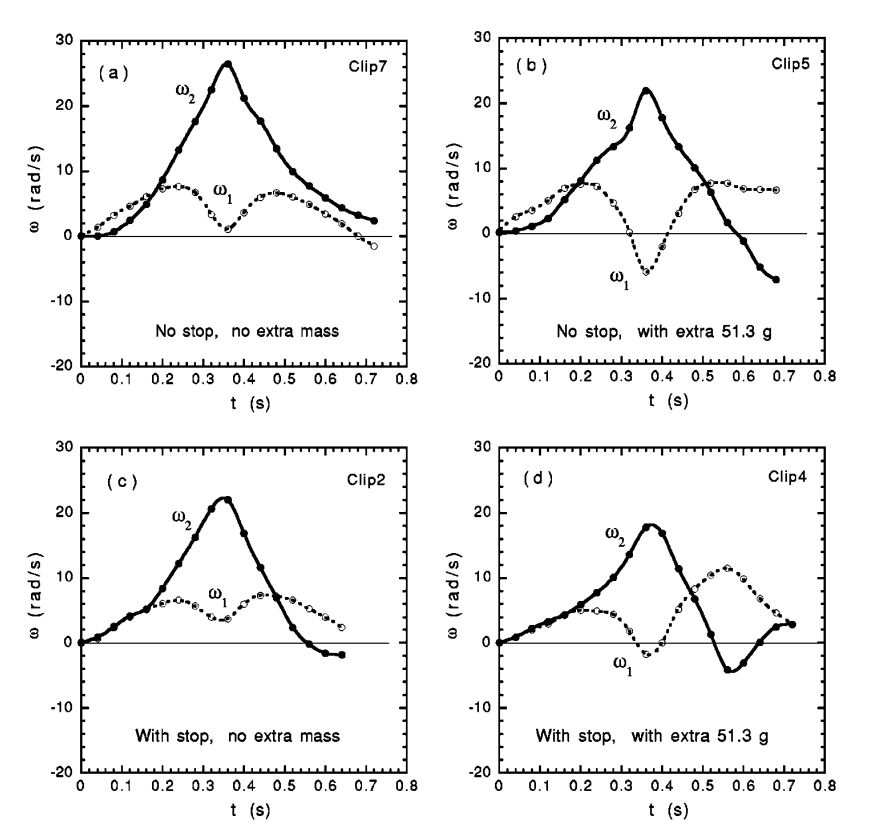
\includegraphics[scale=0.25]{angularvelocities.png}
	\caption{Trials ran for double pendulum with/without stop mechanism and with/without extra 51.3 g mass. The most realistic condition is the trial ran with the stop mechanism and without the added 51.3 g mass (bottom left).}
\end{figure}

Equation 9 was used to solve for the angular velocities of the arm and the rod. The analytical solutions are shown in Figure 8. Comparing these analytical results to Figure 7, the two are highly consistent with one another. There are minor discrepancies that could have been improved with better high speed cameras (used to plot nodes on the double pendulum during its swing) or a lower speed pendulum (that would make the need of a high speed camera irrelevant).

\begin{figure}[H]
	\centering
	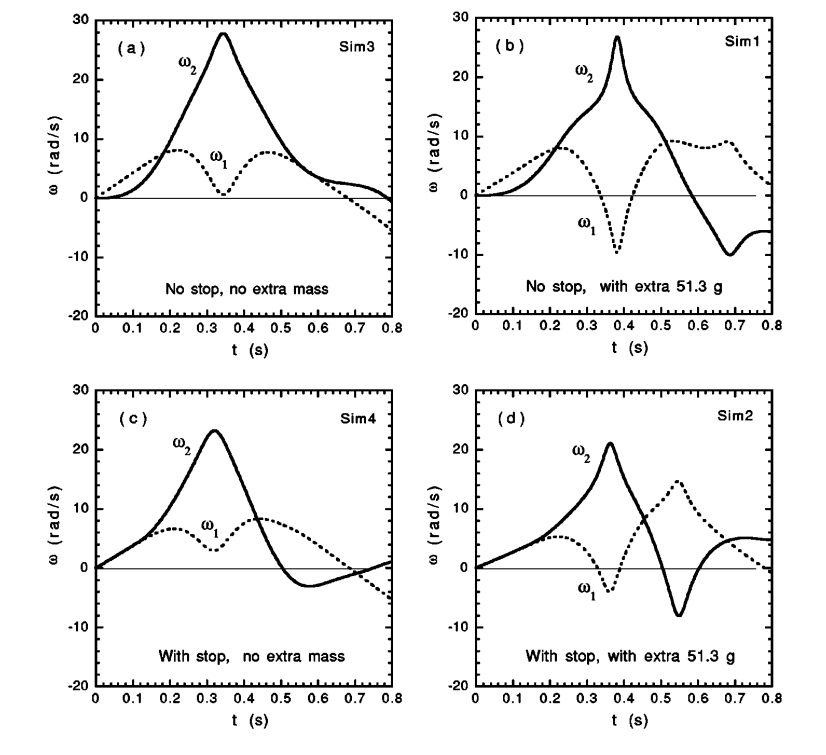
\includegraphics[scale=0.25]{analyticalresults.png}
	\caption{The analytical results for Equation 9, evidently consistent with the experimental results obtained from Figure 7.}
\end{figure}

\section{\label{sec:level4}Force Analysis}

The cause of rotation for the rod segment of the double pendulum can be determined by analyzing the forces acting on it. 


----------
\begin{figure}[H]
	\centering
	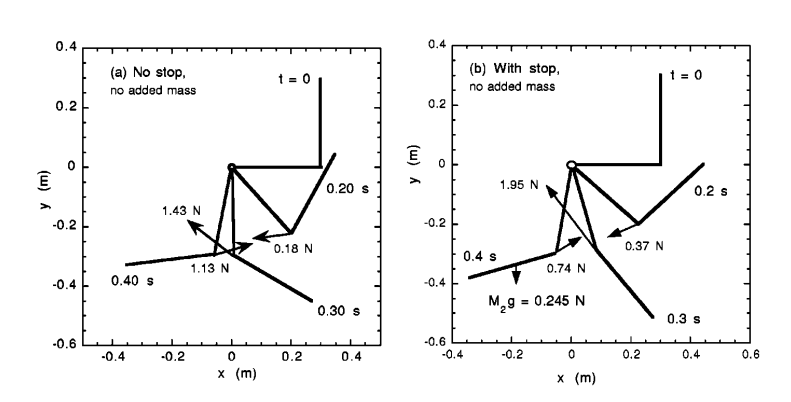
\includegraphics[scale=0.3]{torque.png}
	\caption{}
\end{figure}

\begin{equation}
	F_{\parallel}=\frac{F_x V_x + (F_y - M_2 g) V_y}{V} = M_2 \frac{dV}{dt}
\end{equation}

\begin{equation}
	F_{\perp}=\frac{(F_y - M_2 g)V_x+ F_x V_y}{V} = M_2 \frac{V^2}{R}
\end{equation}

\begin{figure}[H]
	\centering
	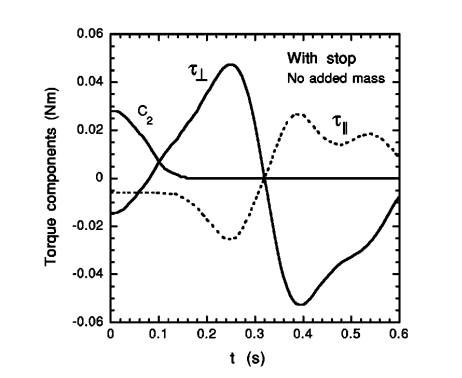
\includegraphics[scale=0.4]{totaltorque.png}
	\caption{}
\end{figure}
		
\begin{equation}
	\tau_{\parallel} = F_{\parallel} h_2 \sin{(\phi - \lambda)}
\end{equation}

\begin{equation}
	\tau_{\perp} = F_{\perp} h_2 \cos{(\phi - \lambda)}
\end{equation}

\begin{equation}
	C_2 + \tau_{\parallel} + \tau_{\perp} = I_{c.m.} \frac{d \omega_2}{dt}
\end{equation}
----------

\section{\label{sec:level5}Energy Transfer}

----------

\begin{figure}[H]
	\centering
	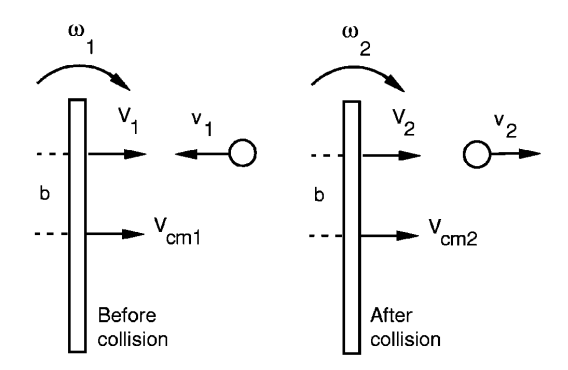
\includegraphics[scale=0.4]{momentumtransfer.png}
	\caption{}
\end{figure}

\begin{equation}
	M V_{c.m.,1} - mv_1 = M V_{c.m.,2} + mv_2
\end{equation}

\begin{equation}
	I_{c.m.} \omega_1 - mv_1b=I_{c.m.} \omega_2 + mv_2b
\end{equation}

\begin{equation}
	e=\frac{v_2 - V_2}{v_1 + V_1} = \frac{v_2 - V_{c.m.,2} - b \omega_2}{v_1 + V_{c.m.,1} + b \omega_1}
\end{equation}

\begin{equation}
	m= \frac{M_e}{[e+(1+e)v_1/V_1]}
\end{equation}
----------

\section{\label{sec:level6}Conclusion}

\nocite{*}
\bibliography{main.bib}% Produces the bibliography via BibTeX.

\end{document}
%
% ****** End of file aipsamp.tex ******
